% !TeX root = ../tesi.tex

\chapter{Oltre la conversazione testuale}

Discuto le ragioni per cui Halue ha proposto questo \emph{stage} e per cui io l’ho scelto. Tratto
il ruolo degli \emph{stage} in azienda, il problema che il progetto affronta, il suo posto nella
strategia di Halue, gli obiettivi e i vincoli fissati dal piano di lavoro e le mie motivazioni.

\section{Il ruolo degli \emph{stage} nella strategia aziendale}
\label{sec:stage-strategia}

Halue ospita in media tre o quattro \emph{stage} all’anno, ed è soprattutto attraverso gli
\emph{stage} che collabora con le università. Gli stagisti provengono per lo più dall’Università di
Padova, dai corsi di laurea triennale e magistrale. L’azienda attribuisce a queste esperienze due
scopi:

\begin{itemize}
	\item svolgere ricerca e sviluppo su temi che i progetti per i clienti non lasciano il tempo di
	esplorare;
	\item conoscere persone da inserire nel \emph{team}, valutando al termine di ogni percorso la
	possibilità di proseguire la collaborazione con lo stagista.
\end{itemize}

Il primo scopo spiega la forma che gli \emph{stage} assumono. Uno stagista lavora a tempo pieno su
un solo tema per circa due mesi, da 300 a 320 ore lavorative, con una continuità che i dipendenti
non hanno, perché l’azienda li ripartisce ogni mese tra più clienti
(\secref{sec:organizzazione-halue}). La quota di tempo che Halue dedica alla ricerca e sviluppo
(\secref{sec:innovazione}) è frammentata, per i dipendenti, tra un progetto e l’altro; in uno
\emph{stage} si concentra invece su un unico tema. Halue affida quindi agli stagisti temi nuovi, su
cui non ha ancora un’esperienza consolidata, e un \emph{tutor} che li segue ogni giorno. Il secondo
scopo spiega perché lo stagista partecipa ai momenti di coordinamento del \emph{team} e ne adotta gli
strumenti, dato che l’azienda valuta il suo modo di lavorare oltre ai risultati che produce.

Alcuni degli \emph{stage} che hanno preceduto il mio riguardavano già gli assistenti
conversazionali. Uno di questi, svolto alcuni anni prima, aveva progettato un assistente basato su
flussi di conversazione predefiniti. In un sistema di questo tipo il progettista definisce in
anticipo gli stati della conversazione e i passaggi tra l’uno e l’altro. A ogni stato l’assistente
riconosce, con un modello addestrato a classificare le frasi, l’intenzione espressa dall’utente, la
associa a uno dei passaggi previsti e gli propone messaggi predefiniti che lo conducono verso una
risposta o un’azione. Il comportamento è deterministico, perché a parità di richiesta l’assistente
segue sempre lo stesso percorso, e una richiesta che il progettista non ha previsto riceve soltanto
una risposta di ripiego.

Un agente basato su un modello linguistico funziona in un altro modo. Il progettista definisce gli
strumenti a disposizione e le istruzioni da seguire, e il modello decide a ogni turno quali
strumenti invocare e come comporre la risposta. Il comportamento diventa non deterministico, perché
la stessa richiesta può ricevere risposte diverse, ma l’agente affronta anche richieste che nessuno
ha previsto. Questo cambiamento, insieme agli strumenti di sviluppo basati sull’IA, ha esteso ciò
che una persona può realizzare nelle ore di uno \emph{stage}. Rispetto a quel progetto, ChatCart
non segue percorsi stabiliti: cerca nel catalogo, compone l’interfaccia e modifica il carrello in
base alla conversazione.
% DA CONFERMARE: lo stage precedente era di Halue? Di che anno?

Ogni \emph{stage} si inserisce in un percorso che lo precede e lo segue. Il tema nasce da
un’esigenza interna oppure dall’interesse che può avere per un laureando in informatica. Nel mio
caso il percorso è iniziato con la candidatura a luglio 2026 e con un colloquio conoscitivo ad
agosto con il \emph{tutor} e con il fondatore. Dopo il colloquio Halue mi ha proposto alcuni temi,
tutti di intelligenza artificiale, tra cui:

\begin{itemize}
	\item uno \emph{storefront} con interfaccia generativa, in cui un agente costruisce la pagina del
	negozio in tempo reale in base a ciò che il cliente cerca;
	\item la gestione del contesto di una base di conoscenza agentica interna all’azienda, cioè un
	archivio di documenti e informazioni aziendali che gli agenti di IA consultano durante il lavoro,
	con un sistema di \gloss{ricerca-semantica}{ricerca semantica} che recupera le informazioni in
	base al loro significato e non soltanto alle parole che contengono;
	\item il monitoraggio dei sistemi di IA in produzione, cioè il controllo del comportamento degli
	agenti già in uso presso l’azienda o i suoi clienti.
\end{itemize}

I temi coprono tutto il ciclo di un sistema di IA: l’esperienza di chi acquista nei negozi dei
clienti di Halue, i processi interni, in cui l’azienda usa già agenti di IA
(\secref{sec:innovazione}), e il funzionamento dei sistemi dopo il rilascio. Ho scelto il primo e
l’ho declinato in un assistente di chat, per le ragioni che espongo nella
\secref{sec:obiettivi-personali}. Ho poi scritto con il \emph{tutor} il piano di lavoro.

Al termine lo stagista presenta il lavoro a tutto il \emph{team} e partecipa a una retrospettiva,
la stessa pratica con cui Halue chiude gli \emph{sprint} e i progetti per i clienti. Il lavoro può
quindi avere due esiti:

\begin{itemize}
	\item l’azienda lo archivia come base di conoscenza sul tema;
	\item l’azienda lo rivede e ne riusa una parte nel codice e nei progetti di produzione.
\end{itemize}

La scelta dipende dal tipo di progetto e dalla qualità del prodotto. Per ChatCart non è ancora
stata presa, e nella \secref{sec:commercio-agentico} descrivo la direzione in cui Halue intende
usarlo.

\section{I limiti degli assistenti conversazionali testuali}
\label{sec:limiti-assistenti}

Molti negozi \emph{online} offrono ai clienti un \gloss{chatbot}{\emph{chatbot}}, un programma che
conversa con l’utente in linguaggio naturale. Di solito compare come
\gloss{widget}{\emph{widget}}, un riquadro sovrapposto alle pagine del negozio che il cliente apre
con un pulsante. Questi assistenti rispondono quasi sempre con solo testo. Il testo è adatto alle
domande frequenti, ma è poco efficace quando il cliente deve confrontare prodotti, scegliere una
taglia o controllare un ordine, cioè nelle operazioni che le pagine di un negozio risolvono con
immagini, prezzi, selettori e pulsanti. Un assistente che descrive a parole tre prodotti costringe
il cliente ad abbandonare la conversazione per vederli, e per il commerciante questo si traduce in
conversazioni che non si concludono con un acquisto. La \figref{fig:confronto} mette a confronto le
due risposte alla stessa richiesta.

\begin{figure}[htbp]
	\centering
	\setstretch{1}
	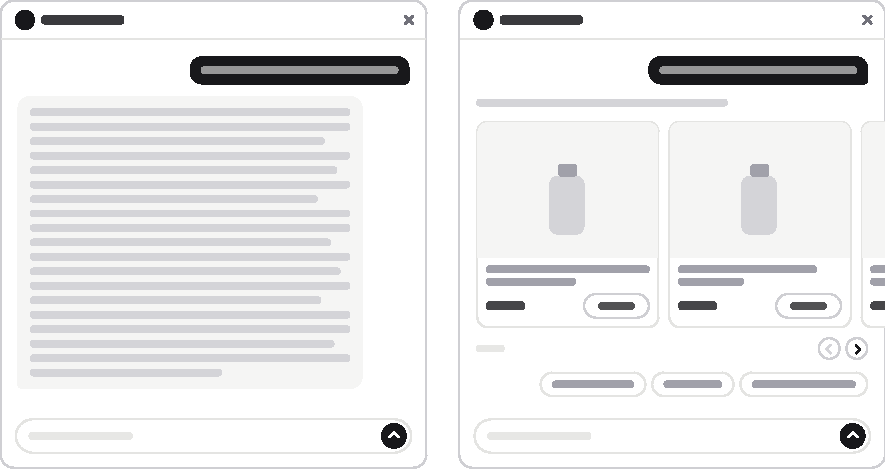
\includegraphics{assets/02-confronto.pdf}
	\caption[Confronto tra un assistente testuale e ChatCart]{\emph{Mockup} della risposta alla
	stessa richiesta di un assistente testuale, a sinistra, e di ChatCart, a destra.}
	\label{fig:confronto}
\end{figure}

Il potenziale di un assistente efficace è misurabile. Uno studio sperimentale condotto tra il 2023
e il 2024 su una delle maggiori piattaforme internazionali di commercio
elettronico\textsuperscript{\ref{rif:studio-genai}} ha confrontato sette applicazioni dell’IA
generativa, ciascuna con un gruppo di clienti che la usava e un gruppo di controllo. L’effetto
maggiore è quello dell’assistente che risponde alle domande dei clienti prima dell’acquisto, che ha
aumentato le vendite del 16,3\%. L’aumento deriva da un numero maggiore di clienti che acquistano,
mentre il valore medio del carrello resta invariato. I clienti che traggono più vantaggio
dall’assistente sono quelli che conoscono meno la piattaforma.

Le soluzioni disponibili sul mercato appartengono a cinque tipi, e ciascuno lascia scoperta una
parte del problema:

\begin{itemize}
	\item \textbf{Gli assistenti generici per l’assistenza clienti} risolvono richieste di supporto
	su più canali a partire dai documenti dell’azienda. Conoscono poco il catalogo e rispondono con
	testo, quindi sono adatti alla gestione di un reso più che alla scelta di un prodotto.
	\item \textbf{Gli assistenti alla vendita preconfezionati} si installano nel negozio e
	consigliano prodotti. L’interfaccia, il modello e il comportamento sono decisi dal fornitore e
	restano uguali per tutti i negozi che li adottano.
	\item \textbf{Sidekick}\textsuperscript{\ref{rif:sidekick}}, l’assistente che Shopify integra nel
	pannello di amministrazione, supporta il commerciante nella gestione del negozio e non si
	rivolge a chi acquista.
	\item \textbf{Il \emph{server} MCP del negozio}\textsuperscript{\ref{rif:storefront-mcp}}, che
	Shopify attiva per ogni negozio, espone agli agenti la ricerca nel catalogo, il carrello e le
	condizioni di vendita. È un componente destinato a chi sviluppa un agente, perché fornisce dati
	e operazioni senza un’interfaccia, e la sua ricerca è la stessa per ogni catalogo.
	\item \textbf{\gloss{ucp}{UCP}}\textsuperscript{\ref{rif:ucp}}, uno standard aperto che Shopify
	e Google hanno pubblicato nel gennaio 2026, permette a un agente di scoprire che cosa offre un
	negozio e di completare un acquisto. È pensato per gli assistenti di terze parti, per cui la
	conversazione avviene fuori dal negozio, in un’interfaccia che il marchio non controlla.
\end{itemize}

Nessuna di queste soluzioni soddisfa insieme i tre requisiti a cui i clienti di Halue attribuiscono
più valore:

\begin{itemize}
	\item l’identità visiva del marchio, perché l’assistente fa parte del negozio e deve avere il suo
	stesso aspetto;
	\item i dati specifici del catalogo, con le varianti, le collezioni e le informazioni che
	distinguono i prodotti di quel marchio;
	\item un’esperienza d’acquisto che si svolge interamente nel negozio, dalla domanda al carrello.
\end{itemize}

Un prodotto preconfezionato deve adattarsi a tutti i commercianti, e per questo lascia poco spazio
alla personalizzazione. Halue costruisce soluzioni per il singolo cliente, perciò ha scelto di
esplorare un assistente su misura basato su un’\gloss{interfaccia-generativa}{interfaccia
generativa}, cioè un’interfaccia che il modello compone durante la conversazione invece di restare
fissata da chi la sviluppa. Il termine comprende approcci che si distinguono per quanto controllo
lasciano al modello:

\begin{itemize}
	\item il modello risponde soltanto con testo, e l’interfaccia resta quella fissa della chat;
	\item il modello sceglie un componente da una libreria predefinita, come una scheda prodotto, e
	lo popola in tempo reale con i dati del negozio, mentre aspetto e comportamento del componente
	restano decisi da chi lo sviluppa;
	\item il modello genera da sé la struttura dell’interfaccia, per esempio sotto forma di codice o
	di una descrizione degli elementi da disporre, e può quindi produrre forme che nessuno ha
	previsto.
\end{itemize}

Halue ha scelto il secondo approccio. Il marchio conserva il controllo sull’aspetto dei
componenti, e il modello decide soltanto quale mostrare e con quali dati. Le scelte del modello
restano non deterministiche, ma ognuna produce un componente progettato e verificato in anticipo:
un errore riguarda al più il componente o i dati scelti, mentre la grafica e il funzionamento dei
pulsanti restano quelli previsti. Il terzo approccio offre più libertà, ma rende difficile garantire
la coerenza con il tema del negozio e la correttezza di prezzi, varianti e pulsanti d’acquisto, che
in un negozio hanno conseguenze dirette sulle vendite.

\section{Il commercio agentico nella visione di Halue}
\label{sec:commercio-agentico}

Il \gloss{commercio-agentico}{commercio agentico} è l’insieme delle esperienze d’acquisto in cui un
agente di intelligenza artificiale accompagna il cliente nella ricerca, nella scelta e
nell’acquisto di un prodotto. Si sta sviluppando in due direzioni:

\begin{itemize}
	\item il negozio si apre ad assistenti generici di terze parti, che lo raggiungono con protocolli
	come MCP e UCP, e il cliente conversa altrove mentre il negozio fornisce catalogo e pagamento;
	\item l’assistente appartiene al marchio e opera all’interno del negozio, con la sua interfaccia
	e con strumenti scritti per il suo catalogo.
\end{itemize}

Le piattaforme promuovono la prima direzione, che un commerciante può adottare senza alcuno
sviluppo dedicato. In questa direzione il negozio diventa una fonte di dati per un assistente che il
marchio non controlla: è l’assistente a decidere come presentare i prodotti, quali proporre accanto
a quello cercato e in quale ordine, e la relazione con il cliente passa per un’interfaccia esterna.
La seconda direzione lascia al marchio questa relazione, ma richiede un progetto su misura per ogni
negozio. ChatCart esplora la seconda.

La scelta è coerente con il modo in cui Halue sta sul mercato. L’azienda lavora su commessa e non
vende prodotti propri (\secref{sec:profilo}), quindi la sua innovazione passa per le competenze che
porta nei progetti dei clienti. Un assistente del
marchio va costruito sul catalogo, sul tema e sui processi di un singolo negozio, cioè sul tipo di
lavoro che Halue svolge già per i suoi clienti Shopify Plus. È la direzione in cui un’azienda delle
sue dimensioni può offrire un servizio che le piattaforme non coprono, e in cui può far valere ciò
che conosce dei negozi che segue. Halue si colloca tra le aziende che lavorano già in modo concreto
sull’intelligenza artificiale per il commercio elettronico, e con questo \emph{stage} cerca di
estendere quella competenza a un prodotto rivolto al cliente finale.

Prima dello \emph{stage} Halue disponeva già di alcune premesse:

\begin{itemize}
	\item i negozi realizzati per marchi che vendono su più mercati, con le loro integrazioni
	(\secref{sec:clientela});
	\item gli agenti collegati ai dati dei negozi con strumenti propri e quelli che usa per i processi
	interni (\secref{sec:innovazione});
	\item la consulenza e la formazione sull’intelligenza artificiale per i clienti, dalla
	valutazione della loro preparazione ai \emph{workshop} del fondatore (\secref{sec:profilo}).
\end{itemize}

Non aveva invece esperienza su un assistente rivolto al cliente finale, che pone problemi diversi
da quelli di un agente a uso interno perché deve integrarsi con il tema del negozio, rispondere in
pochi secondi e comportarsi in modo prevedibile con qualsiasi interlocutore. Lo \emph{stage} aveva
lo scopo di costruire questa competenza su un caso sufficientemente circoscritto da poter essere
completato nella durata prevista.

Al termine dello \emph{stage}, il risultato costituisce per l’azienda una base di ricerca e
sviluppo. L’obiettivo dichiarato è arrivare a proporre questo tipo di soluzione ai clienti come
servizio, con tempi e forma ancora da stabilire. Il primo passo è stata la presentazione al
\emph{team} del 9 novembre 2026, l’ultimo giorno di \emph{stage}, articolata in trenta minuti
dedicati al prodotto, quindici alla parte tecnica e quindici alle domande. Le domande hanno
mostrato quali aspetti interessano a chi riprenderà il lavoro, in particolare le scelte di
progettazione, come la gestione dello stato nella sincronizzazione del carrello, e il modo in cui
ho istruito l’agente perché si comportasse come previsto.

\section{Obiettivi e vincoli del progetto}
\label{sec:obiettivi}

Il piano di lavoro, che ho scritto con il \emph{tutor} ad agosto 2026, organizza il prototipo su
due livelli (\figref{fig:livelli}). L’\emph{app layer} è il \emph{widget} di chat nel negozio e si
limita a visualizzare la conversazione e i componenti. L’\emph{agent layer} è il \emph{backend},
cioè il programma eseguito su un \emph{server}, che ospita l’agente e conserva lo stato della
conversazione. Per interrogare le API di Shopify l’agente usa il
\gloss{tool-calling}{\emph{tool calling}}, il meccanismo con cui un modello linguistico chiede al
programma che lo ospita di eseguire una funzione e ne riceve il risultato.

\begin{figure}[htbp]
	\centering
	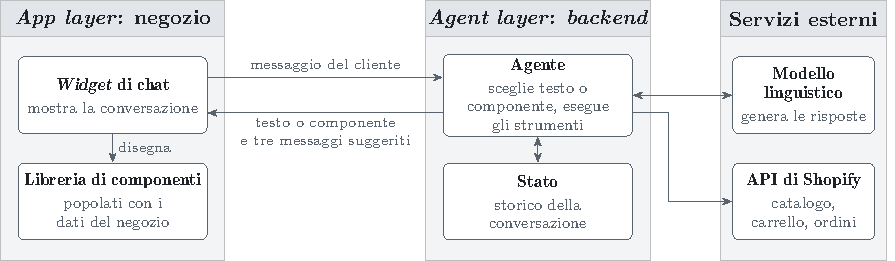
\includegraphics{assets/02-livelli.pdf}
	\caption[L’architettura su due livelli prevista dal piano di lavoro]{L’architettura su due
	livelli prevista dal piano di lavoro. Il \emph{widget} non contiene logica conversazionale: ogni
	decisione spetta all’agente, che può interrogare più volte modello e API prima di rispondere.}
	\label{fig:livelli}
\end{figure}

Gli obiettivi hanno un identificativo, che uso nel resto della relazione, e tre livelli di
priorità. Gli obiettivi obbligatori (\tabref{tbl:obbligatori}) sono vincolanti e, oltre a
dimostrare la fattibilità dell’approccio, chiedono di misurarne l’efficacia.

Gli obiettivi desiderabili hanno un valore aggiunto riconoscibile, quelli facoltativi un valore
aggiunto non prioritario (\tabref{tbl:desiderabili}). Riprendono tre aspetti che il \emph{tutor}
ha indicato come interessanti per l’azienda: il supporto a più mercati, i temi Hydrogen, in cui il
riuso dei componenti React è più semplice e l’integrazione con il carrello più complessa, e una
ricerca nel catalogo scritta su misura, perché il \emph{tutor} giudicava elementare quella del
\emph{server} MCP di Shopify.

\begin{tabellatesi}{P{0.1}P{0.9}}
	{Gli obiettivi obbligatori del piano di lavoro.}
	{tbl:obbligatori}
	\toprule
	\rowcolor{TabellaIntestazione} \textbf{ID} & \textbf{Obiettivo} \\
	\midrule
	OB1 & \emph{App layer}: \emph{widget} di chat in React e TypeScript integrato nel negozio \\
	OB2 & \emph{Agent layer}: \emph{backend} Node.js con un agente dotato di \emph{tool calling}, in
	grado di interrogare le API di Shopify \\
	OB3 & Risposte in linguaggio naturale (domande generali, sui prodotti, di chiarimento) oppure con
	un componente predefinito, scelto e popolato in base alla conversazione \\
	OB4 & Libreria di almeno due o tre componenti flessibili e tre messaggi suggeriti per ogni
	risposta \\
	OB5 & Raccolta di metriche di coinvolgimento e di conversione sull’uso del \emph{widget} \\
	\bottomrule
\end{tabellatesi}

\begin{tabellatesi}{P{0.1}P{0.2}P{0.7}}
	{Gli obiettivi desiderabili e facoltativi del piano di lavoro.}
	{tbl:desiderabili}
	\toprule
	\rowcolor{TabellaIntestazione} \textbf{ID} & \textbf{Priorità} & \textbf{Obiettivo} \\
	\midrule
	DE1 & desiderabile & Supporto a \gloss{shopify-markets}{Shopify Markets}, la funzione con cui un
	negozio vende in più paesi con lingue e valute diverse \\
	DE2 & desiderabile & Componente per lo stato dell’ordine e il supporto dopo la vendita \\
	FA1 & facoltativo & Prova di fattibilità dell’integrazione su Hydrogen, con il riuso dei
	componenti del \emph{widget} \\
	FA2 & facoltativo & Confronto sperimentale tra la ricerca su misura, il \emph{server} MCP di
	Shopify e un eventuale \emph{server} MCP proprio \\
	\bottomrule
\end{tabellatesi}

Gli obiettivi traducono in prodotto i requisiti della \secref{sec:limiti-assistenti}. OB1 porta
l’assistente dentro il negozio, così che l’esperienza d’acquisto non ne esca. OB2 collega l’agente
ai dati reali del catalogo invece che alla memoria del modello, secondo la prima delle regole di
Halue per i progetti di IA (\secref{sec:innovazione}). OB3 e OB4 realizzano l’interfaccia
generativa con componenti predefiniti, che rispettano l’identità visiva del marchio, e DE1 estende
lo stesso comportamento ai negozi che vendono su più mercati, come quelli dei clienti di Halue.
OB5 serve a verificare se l’assistente produce il beneficio che lo studio citato nella
\secref{sec:limiti-assistenti} attribuisce a un assistente efficace, cioè più clienti che arrivano
all’acquisto.

Per l’azienda il criterio di successo era un prototipo funzionante dall’inizio alla fine su un
negozio di esempio, accompagnato da una valutazione onesta di ciò che funziona e di ciò che non
funziona. Valuto il grado di soddisfacimento di ogni obiettivo nella \secref{sec:soddisfacimento}.

Il progetto aveva i seguenti vincoli, ciascuno con una conseguenza sul lavoro:

\begin{itemize}
	\item \textbf{Quantità di lavoro}: da 300 a 320 ore, con una distribuzione al massimo a tempo
	pieno, dal 14 settembre al 9 novembre 2026. La durata fissa obbligava a scegliere presto che cosa
	approfondire e che cosa lasciare agli sviluppi futuri.
	\item \textbf{Luogo di lavoro}: da remoto, con un giorno a settimana in sede, un allineamento
	quotidiano con il \emph{tutor} e una riunione settimanale di un’ora. Gran parte del confronto
	passava quindi per brevi riunioni a distanza e per i messaggi su Slack.
	\item \textbf{Tecnologie}: TypeScript in tutto il progetto, dal \emph{widget} al \emph{backend}.
	Il piano rimandava alle prime settimane la scelta degli strumenti per costruire l’agente e del
	modello linguistico, che il \emph{tutor} ha lasciato a me.
	\item \textbf{Piattaforma}: prima i temi Liquid, che sono i più diffusi, e Hydrogen soltanto come
	eventuale approfondimento finale. Il \emph{widget} doveva quindi funzionare all’interno di temi
	che non avevo scritto io.
	\item \textbf{Ambiente}: un unico negozio di sviluppo, senza clienti né traffico reali, con due
	temi installati per le prove. L’ho allestito come un negozio di cosmetica botanica con circa
	quaranta prodotti, perché il comportamento di un assistente dipende dal catalogo su cui opera, e
	varianti, collezioni, confezioni regalo, prodotti esauriti e archiviati lo avvicinano a un caso
	reale. Senza traffico reale, le metriche di OB5 si possono raccogliere soltanto dalle prove.
	\item \textbf{Natura del prodotto}: un prototipo di ricerca e sviluppo, essenziale ma solido,
	senza i requisiti di scala e di costo di un prodotto in produzione. Per questo non ho ottimizzato
	il consumo di \emph{token} né la capacità di servire molti negozi insieme.
\end{itemize}

Il piano ripartisce 310 ore indicative tra dieci attività (\figref{fig:piano}) e prevede che la
ripartizione sia rifinita con il \emph{tutor} nelle prime settimane. Nella
\secref{sec:pianificazione} la confronto con l’uso effettivo del tempo.

\begin{figure}[htbp]
	\centering
	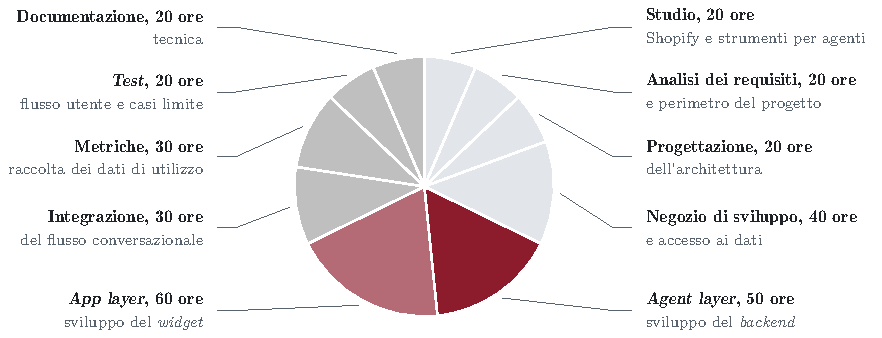
\includegraphics{assets/02-piano.pdf}
	\caption[La ripartizione delle ore prevista dal piano di lavoro]{La ripartizione delle ore
	prevista dal piano di lavoro, in senso orario dall’alto. In grigio chiaro le attività che
	precedono la scrittura del codice, in bordeaux lo sviluppo dei due livelli, in grigio medio le
	attività che lo completano.}
	\label{fig:piano}
\end{figure}

\section{Motivazioni e obiettivi personali}
\label{sec:obiettivi-personali}

Da marzo 2026 lavoro in proprio come sviluppatore di negozi Shopify. Il mio cliente principale è
Dr Kampes, un marchio per cui ho svolto compiti molto diversi tra loro: ho creato e configurato il
negozio, gestito e ampliato il catalogo, impostato le regole di spedizione, realizzato lo
\emph{storefront} e collegato il CRM, con le automazioni che seguono l’acquisto e quelle di
\emph{marketing}. Questo lavoro mi ha dato una visione ampia della piattaforma, ma non mi ha
permesso di specializzarmi in un ambito. Riguardava inoltre soltanto i temi Liquid, e mai lo
sviluppo di applicazioni.
% DA CONFERMARE: Dr Kampes è un marchio di calzature? Serve una voce nei Riferimenti?

Prima di scegliere Halue ho sostenuto un colloquio conoscitivo con un’altra azienda, esterna alle
offerte dell’ateneo, e ho letto le altre proposte di \emph{stage}. Queste erano pensate per il
lavoro in aziende grandi e strutturate, mentre io preferisco progetti piccoli e di nicchia, che
lasciano spazio alla sperimentazione e a iterazioni rapide. La proposta di Halue rispondeva a
questa preferenza e aveva tre vantaggi:

\begin{itemize}
	\item riguardava Shopify, la piattaforma su cui già lavoravo, in un’azienda che la usa ogni
	giorno, e mi permetteva di passare dall’uso dei suoi strumenti alla costruzione di applicazioni;
	\item mi offriva due mesi a tempo pieno su tecnologie che mi interessavano già, un’occasione che
	il lavoro in proprio difficilmente concede;
	\item già al colloquio Halue mi ha proposto di lavorare soprattutto da remoto, una condizione
	decisiva, perché la sede dista circa un’ora e mezza di auto da casa mia.
\end{itemize}

Tra i temi proposti ho scelto l’interfaccia generativa. La gestione del contesto mi
interessava molto e apriva diverse strade di integrazione con altri strumenti e sistemi, ma
comportava un rischio. I grandi fornitori di modelli linguistici aggiornano i propri assistenti a
ritmo serrato, e funzioni come la ricerca nei documenti e negli strumenti di un’azienda entrano in
quegli assistenti una dopo l’altra. Un sistema costruito in due mesi rischiava di essere superato
da un aggiornamento di un assistente generico. Un assistente di vendita dentro il negozio di un
marchio dipende invece da elementi che solo quel negozio possiede, cioè il suo catalogo, il suo
tema e il suo carrello, ed è quindi un bisogno che un assistente generico copre con più difficoltà.

L’idea dell’interfaccia generativa è di Halue, che la proponeva come uno \emph{storefront}
costruito in tempo reale da un agente. Vi ho riconosciuto l’esigenza di Dr Kampes, che mi aveva
parlato di un assistente capace di dare assistenza ai visitatori del negozio e di indirizzarli
verso l’acquisto. Ho quindi proposto di declinare il tema in un assistente di chat che sceglie e
popola componenti dell’interfaccia con i dati del negozio, come schede prodotto, tabelle di
confronto, guide alle taglie e lo stato di un ordine, per accompagnare il cliente dalla scoperta
dei prodotti all’assistenza dopo la vendita. Un assistente di questo tipo si aggiunge al tema di
un negozio esistente invece di sostituirlo, e si può quindi applicare anche ai negozi che Halue e io
seguiamo già.

Il tema toccava anche altri miei interessi:

\begin{itemize}
	\item imparare a sviluppare applicazioni Shopify, per estendere gli \emph{storefront} con
	soluzioni su misura;
	\item collegare i negozi ai miei agenti di IA attraverso le Storefront API e le Admin API
	(\secref{sec:ecosistema});
	\item conoscere la piattaforma più a fondo, capendo come i suoi componenti si incastrano, per
	costruire da zero ciò che finora avevo soltanto usato.
\end{itemize}

Volevo infine mettere alla prova in un progetto reale ciò che ho imparato nel corso di studi: i
\gloss{design-pattern}{\emph{design pattern}}, cioè soluzioni riconosciute a problemi ricorrenti di
progettazione, il rigore nella pianificazione e una progettazione che favorisce le estensioni
future e la manutenzione nel tempo. Lo studio del C++ mi ha mostrato il valore dei linguaggi
tipati, in cui il compilatore controlla i tipi dei dati prima dell’esecuzione. Per questo nel piano
ho proposto TypeScript, che aggiunge i tipi statici a JavaScript, in tutto il progetto.

Il progetto aveva quindi per me un valore che andava oltre lo \emph{stage}. Da queste ragioni ho
ricavato quattro obiettivi personali (\tabref{tbl:personali}), che valuto insieme a quelli del
piano nella \secref{sec:soddisfacimento}.

\begin{tabellatesi}{P{0.1}P{0.9}}
	{I miei obiettivi personali per lo \emph{stage}.}
	{tbl:personali}
	\toprule
	\rowcolor{TabellaIntestazione} \textbf{ID} & \textbf{Obiettivo} \\
	\midrule
	OP1 & Estendere le mie competenze su Shopify dai temi allo sviluppo di applicazioni \\
	OP2 & Acquisire esperienza nella progettazione di sistemi basati su agenti \\
	OP3 & Ricavare dal progetto conoscenze e soluzioni riutilizzabili nella mia attività
	professionale \\
	OP4 & Gestire in autonomia il lavoro da remoto, dove nessuno segue la mia giornata in modo
	continuo e spetta a me organizzarla, stabilire le priorità e prevedere le pause \\
	\bottomrule
\end{tabellatesi}
